\begin{table}[!t]
\begin{threeparttable}
\caption{Performance at comparable data size and different logical-domain size.}
\label{table:experiment}
%\renewcommand{\TPTnoteSettings}{\footnotesize}
	% \begin{tabular*}{\columnwidth}{@{} l r r}
	\begin{tabular*}{\columnwidth}{@{\extracolsep{\fill}} l r r}
	\toprule
	& \quad Homogeneous
	%Multiplications
	& \quad Heterogeneous
		\\
	% & \multirow{2}{*}{\makecell{Memory \\ Usage}} 
	\midrule
	Input entries $N$ & $2^{34}$ & $2^{34}+1$ \\
	\hline
	Logical domain $K$ & $2^{34}$ & $2^{35}$ \\
	\hline
	Dense $K$-domain witness\tnote{a} & $512$\,GiB & $1$\,TiB \\
	\hline
	Evaluation time & $208.06$ s & $280.22$ s  \\ 
	\hline
	Setup time & $6.84$ s & $7.73$ s  \\ 
	\hline
	Commit time & $1,727.64$ s & $1,761.87$ s  \\ 
	\hline
	Commit size & $576$ B & $576$ B  \\ 
    \hline
	Value\&point commit time & $0.16$ s & $0.26$ s  \\ 
	\hline
	Value\&point commit size & $576$ B  & $576$ B  \\ 
	\hline
	Open time & $360.14$ s & $383.75$ s  \\
	\hline
	   \quad Inner product proof & $254.99$ s & $247.55$ s \\
	   \quad Proof of TBV evaluation & $0.75$ s & $0.67$ s \\
	   \quad Base PCS opening & $104.38$ s & $135.45$ s  \\
    \hline
    Proof size & $101.81$ KB & $103.03$ KB  \\
		\hline
	Verifier time & $0.30$ s & $0.33$ s \\
		\hline
	Peak RAM & $291.85$ GB & $404.41$ GB  \\
	\bottomrule
\end{tabular*}
\begin{tablenotes}[para, flushleft]
	\item[a] Estimated at 32 bytes per field element; this dense representation is not allocated.
	\item Parallelized across $64$ CPU threads except for verifier algorithms.
\end{tablenotes}
\end{threeparttable}
\end{table}

\section{Experimental Evaluation}
\label{sec:experiments}

We implement the collection-commitment construction in Rust and evaluate its
prover time, verifier time, proof size, and peak RAM in a fully virtualized
x86\_64 environment exposing 90 logical CPU threads and equipped with
512\,GiB of RAM.
The virtual CPUs report an Intel Core i7-8700K model running at 3.70\,GHz.
Except for verifier algorithms, we use 64 threads for parallelization.\footnote{
Our code is available at \url{https://anonymous.4open.science/r/hdr1cs-0311}.
}
Table~\ref{table:experiment} summarizes the experimental results.

\mysmallskip
{\bf Base PCS.}
We instantiate the construction using a variant of Dory~\cite{tcc/Lee21},
a folding-based polynomial commitment scheme over pairing groups on BLS12-381.
We choose this PCS because its measured memory usage is the lowest among the
implementations in Table~\ref{table:experimentPCS}, and because it supports
blockwise commitment and opening (Appendix~\ref{appx:pcs}).
The prover time of our PCS scales linearly with the bit-width of the witness.
Since we are motivated by zkML and modern NNs commonly adopt 8-bit quantization~\cite[\S~1]{corr/micikevicius22},
we conduct experiments on 8-bit vectors.
The collection layer can also be instantiated with other PCSs that expose
bucket-wise commitment and opening, including BaseFold
~\cite{crypto/ZeilbergerCF24}.

\mysmallskip
{\bf Heterogeneous vs.\ homogeneous vectors.}
We evaluate heterogeneous and homogeneous collections at $2^{34}$ scale,
approximately $17.2$ billion entries.  This is comparable to the parameter scale
of the LLaMA2-13B model~\cite{arxiv/Llama23} and provides a large zkML-shaped
packing workload.

In the heterogeneous setting, we use $36$ vectors with sizes:
\[
  \{1, 1, 1, 2, 2^2, 2^3, \ldots, 2^{33}\}.
\]
Following the BVA layout rule, the $36$ real buckets are ordered by decreasing
size.  Their cover length is $S=N=2^{34}+1$; the logical domain has
$K=2^{35}$ and one implicit trailing zero suffix of length $2^{34}-1$.
Padding all $36$ vectors to the maximum length would instead create
$36\cdot2^{33}$ slots, about $18\times$ the exact unpadded length
$N=2^{34}+1$.  Storing that maximum-padded domain as 32-byte field elements
would require 9\,TiB.  BVA's logical domain has length $2^{35}<2N$, whose dense
field representation would still require 1\,TiB, but none of its $2^{35}-N$
padded coordinates is materialized.  This workload directly measures the
separation between logical domain expansion and physical prover storage.

In the homogeneous setting, we round the vector count up to the next power of two,
\ie, $64$, which is more favorable for folding-based protocols.
All vectors have an equal size of $2^{28}$.
In this case, $S=K=2^{34}$, so there is no final zero suffix.

We compare the performance of these two settings in
Table~\ref{table:experiment}.  Both contain approximately $2^{34}$ real entries,
but the heterogeneous logical domain is twice as large.  Nevertheless, prover
time is nearly identical ($\sim29$ min for commitment and $\sim6$ min for
opening), with proof size around $100$\,KB and verifier time about $0.3$ s.
The peak RAM usage is $292$\,GB for the homogeneous setting
and $404$\,GB for the heterogeneous setting.

For reference, storing $2^{34}$ entries as 256-bit field elements requires
512\,GiB.  Our memory footprint is lower because we store witnesses in 8-bit
format and convert them to field elements bucket by bucket.
In the heterogeneous setting, the presence of a single large bucket of size $2^{33}$
(which alone corresponds to 256\,GB when materialized as field elements)
leads to higher peak RAM usage.

The heterogeneous run stays within $404.41$\,GB peak RAM even though a dense
representation of its logical domain would require 1\,TiB for the witness
alone.  The inner-product proof traverses stored entries rather than conceptual
zeros; accordingly, its time is $247.55$ s in the heterogeneous experiment and
$254.99$ s in the homogeneous experiment despite the former's twice-as-large
logical domain.  The result isolates the intended effect: padding changes the
algebraic domain but does not add folding work.

\mysmallskip
{\bf Scaling with total vector size and vector count.}
We further study the scalability of the construction with respect to
the total vector size $N$ and the vector count $T$.
In zkML scenarios,
$N$ corresponds to the total parameter size,
while $T$ is the number of committed parameter vectors.

Figure~\ref{fig:experiment} reports the commitment time, opening time,
proof size, and verifier time as $N$ and $T$ vary.
The observed behavior matches our analysis: commitment and opening times scale
linearly with $N$ and are largely independent of $T$, while proof size and
verifier time grow logarithmically in $N$ and $T$.  Vector count affects the
compact metadata term rather than introducing work proportional to a common
maximum-sized domain.
Opening time is irregular for small $T$ because the implementation disables
parallelization for vectors smaller than $2^{10}$.

\begin{figure}[!t]
\centering
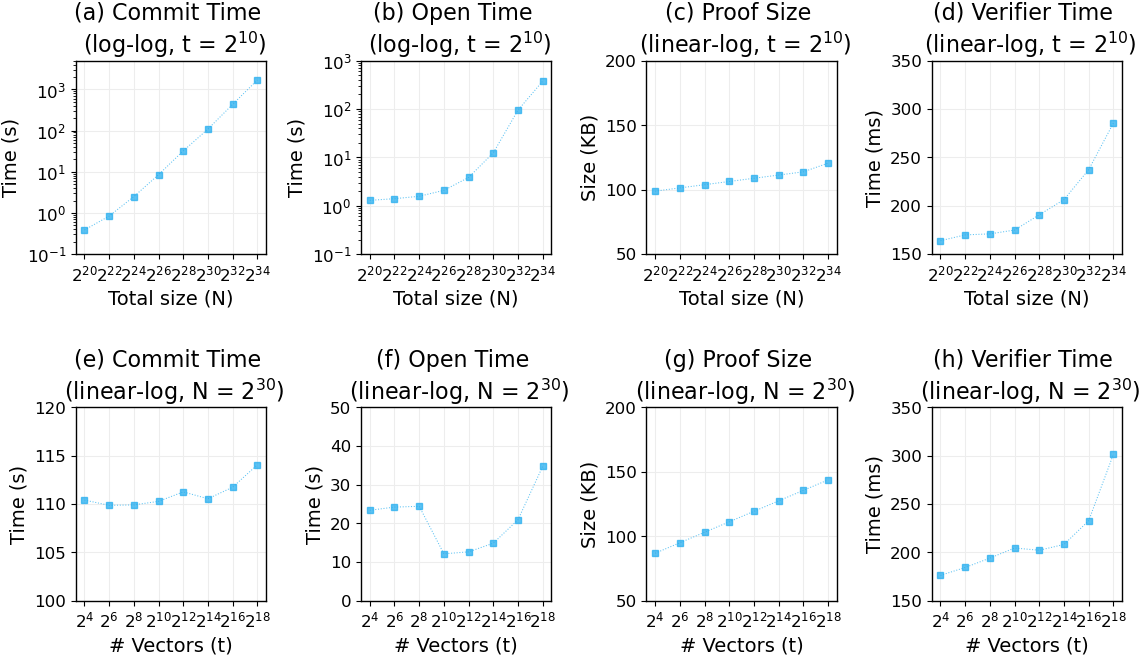
\includegraphics[width=\linewidth]{figure/experiment.png}
\caption{
Performance under
(i) varying total size $N$ with fixed vector count $T$, and
(ii) varying $T$ with fixed total size $N$.
} 
\Description{Experimental results.}
\label{fig:experiment}
\end{figure}
